\documentclass[border=6pt]{standalone}
\usepackage{amsmath}
\usepackage{tikz}
\usetikzlibrary{positioning, arrows.meta, fit, backgrounds, calc}
\tikzset{stage/.style={draw, rounded corners, align=center, font=\small, minimum height=1.0cm, minimum width=2.6cm, thick},
layer/.style={draw, dashed, rounded corners, inner sep=10pt},
node_t/.style={draw, circle, align=center, font=\scriptsize, minimum size=1.0cm, thick},
flow/.style={-{Stealth[length=2.5mm]}, thick},
edge_t/.style={-{Stealth[length=2mm]}, font=\scriptsize}}
\begin{document}
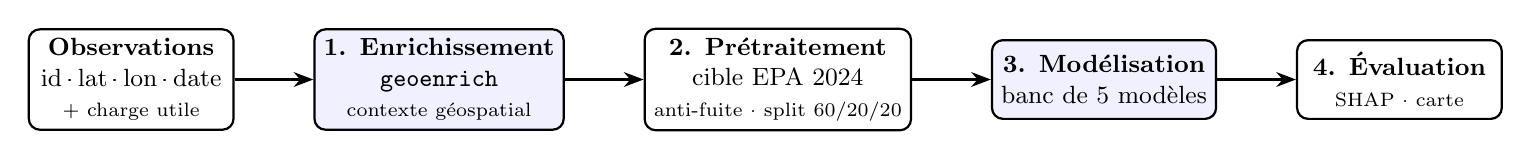
\begin{tikzpicture}[node distance=0.9cm and 1.0cm]
  \node[stage] (a) {\textbf{Observations}\\ id\,·\,lat\,·\,lon\,·\,date\\ {\scriptsize+ charge utile}};
  \node[stage, right=of a, fill=blue!6] (b) {\textbf{1. Enrichissement}\\ \texttt{geoenrich}\\ {\scriptsize contexte géospatial}};
  \node[stage, right=of b] (c) {\textbf{2. Prétraitement}\\ cible EPA 2024\\ {\scriptsize anti-fuite · split 60/20/20}};
  \node[stage, right=of c, fill=blue!6] (d) {\textbf{3. Modélisation}\\ banc de 5 modèles};
  \node[stage, right=of d] (e) {\textbf{4. Évaluation}\\  {\scriptsize SHAP · carte}};
  \draw[flow] (a) -- (b);
  \draw[flow] (b) -- (c);
  \draw[flow] (c) -- (d);
  \draw[flow] (d) -- (e);
\end{tikzpicture}

\end{document}
